 \section{РАСЧЁТ УЗЛОВ ПРЕДВАРИТЕЛЬНОГО УСИЛЕНИЯ}

 \textbf{\subsection{Расчет мостового регулятора тембра}}
  \vspace{1em}
 
 Регулятор тембра служит для коррекций частотной характеристики всей схемы, а также приданию звуку желаемой окраски. \par

\begin{figure}[!htbp]
    \center{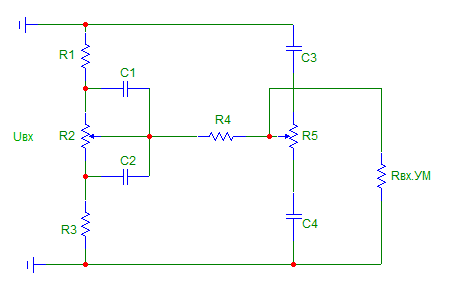
\includegraphics[width=0.6\linewidth]{picture_cor}}
    \caption{Схема мостового регулятора тембра}
    \label{figure:p3_4}
  \end{figure}

 Цепочка R1, R2, R3 и C1, C2 – регулятор низких частот. \par
Цепочка R5, С3, С4 – регулятор высоких частот.
Входной каскад усилителя мощности имеет малое входное сопротивление, ограниченное R1. Особенностью пассивного регулятора тембра является то, что эти регуляторы требуют низкого выходного сопротивления предшествующего им каскада и высокого входного сопротивления последующего. По этой причине входной каскад УМ и регулятор тембра РТ отделяют каскадом предварительного усиления, выполненного по схеме с общим коллектором, входное сопротивление которого имеет большую величину, а выходное – малую. Это обеспечивает их совместимость и не потерю сигнала. Нагрузкой для регулятора тембра является входное сопротивление каскада предварительного усиления.

\subsubsection{Коэффициент коррекции:} % (fold)

 \begin{equation}
  \label{eq:equation5_1}
  m \geq 10^{ \left| \Delta b_{\text{т}}  
   \right| /20 }
\end{equation}
\begin{equation*}
  m \geq 10^{ \left| \pm 14.0  \right| /20 } = 5.012
\end{equation*}

% subsubsection коэффициент_коррекции_ (end)

\subsubsection{Частота раздела определяется:} % (fold)
  
  \begin{equation}
    \label{eq:equation5_2}
      f_0 = \sqrt{f_{\text{н}} \cdot f_{\text{в}}} = \sqrt{ 10\cdot 18000} = 424~\text{Гц}
   \end{equation} 

% subsubsection subsubsection_name (end)

\subsubsection{Условие неперекрытия зон регулирования:} % (fold)
Одним уз существенных условий нормального функционирования регулятора тембра является расположение частоты нижнего и верхнего среза на расстоянии, обеспечивающим их неперекрытие. Т.е. чтобы избежать взаимного влияние низкочастотного и высокочастотного регуляторов. \par

  \begin{equation}
    \label{eq:equation5_3}
      2 m f_{\text{н}} \leq f_0 \leq \dfrac{f_{\text{в}}}{2m} 
 \end{equation} 
 \begin{equation}
   \label{eq:equation5_4}
    100 \leq f_0 \leq 1796
  \end{equation} 

    Т.о. видно, что не происходит взаимного влияния низкочастотного и высокочастотного регулятора.

% subsubsection subsubsection_name (end)

\subsubsection{Сопротивления подстроечных резисторов R = R2 = R5:}
\begin{equation}
   \label{eq:equation5_5}
	R=0.5 \cdot R_{\text{ВХ СЛ}}=0.5 \cdot R_{\text{ВХ КПУ 2}}=0.5 \cdot  4429=1175.2~\text{кОм}
\end{equation} 

\subsubsection{ Номиналы регистров регулирования НЧ:}
\begin{equation}
   \label{eq:equation5_6}
   R_1=\dfrac{R}{m}=1175192 /5 =1050581~\text{Ом}
   \end{equation} 
   \begin{equation}
   \label{eq:equation5_7}
   R_3=\dfrac{R_1}{m}=1050581 / 5=2776~\text{Ом}
   \end{equation} 
   \subsubsection{ 6. Сопротивление буферного  резистора R4.}
   Буферный резистор обеспечивает развязку  низкочастотного и высокочастотного регуляторов. 
   \begin{equation}
   \label{eq:equation5_8}
   R_4=(0.05 \ldots 0.1) \cdot R=(0.05 \ldots 0.1) \cdot 1175192 \cdot 10^3 = 221~\text{Ом}
   \end{equation} 
   \subsubsection{    Задание номинальных значений емкостей.}
   Емкости в схеме регулятора тембра обеспечивают его работу как фильтра.
   \begin{equation}
   \label{eq:equation5_9}
   C_1=\dfrac{1}{2 \pi \cdot f{\text{Н}}\cdot m \cdot R}  \cdot=\dfrac{1}{2 \cdot \pi \cdot 10 \cdot 5 \cdot 1175192 \cdot 10^3}=1434.06~\text{нФ}
   \end{equation} 
   \begin{equation}
   \label{eq:equation5_10}
   C_2=m \cdot C_1=5 \cdot 1434.06= 7187~\text {нФ}
   \end{equation} 
        Емкости С3 и С4 формируют ВЧ-регулятор.
        \begin{equation}
   \label{eq:equation5_11}
   C_3=\dfrac {m^2}{(4\cdot \pi \cdot f_{\text{в}}\cdot m \cdot R) }= 5^2/(4 \cdot \pi \cdot 18000 \cdot 1175192 )= 50.15~\text{нФ}
   \end{equation} 
  \begin{equation}
   \label{eq:equation5_12}
  C_4=m \cdot C_3=5 \cdot 50.15=251~\text{нФ}
  \end{equation} 
\subsubsection{   Задание входного и выходного сопротивления регулятора тембра.   }
\begin{equation}
   \label{eq:equation5_13}
R_{\text{ВХ T}}=R_1+R_3=1050581+2776=277309~\text{Ом}
\end{equation} 
\begin{equation}
   \label{eq:equation5_14}
   R_{\text{ВЫХ Т}}=R_4+\dfrac{R_1 \cdot R_3}{R_1+R_3} = 221+1050581 \cdot 2776 /(1050581+2776)=295~\text{Ом}
   \end{equation}

\subsubsection{ Определение требования к выходному сопротивления предыдущего каскада   }

\begin{equation}
   \label{eq:equation5_15}
   R_{\text{ВЫХ ПРЕД}}=0.2 \cdot R_{\text{ВХ Т}}=0.2 \cdot 295 = 59 ~\text{Ом}
\end{equation}
Выходное сопротивление предшествующего каскада для регулятора тембра представляет собой эквивалентное сопротивление генератора сигнала. Для согласования каскада и передачи сигнала с минимальными потерями оно выбирается в 5…10 раз меньше входного сопротивления регулятора тембра.

\subsubsection{ Определение положения движков R2 и R5, соответствующие линейной частотной характеристике:}

  \begin{equation}
  \label{eq:equation5_16}
  R^{''}=\dfrac{R \cdot m}{m^2-1}=1175192  \cdot  5/(5-1)=460~\text{Ом}
  \end{equation}

  \begin{equation}
  \label{eq:equation5_17}
  R^{'}=R-R^{''}=1175192  -460 =1.75 ~\text{кОм}
  \end{equation}

  \subsubsection{ Номинальный коэффициент передачи тембра на средних частотах имеет вид:}
   
  \begin{equation}
  \label{eq:equation5_18}
   K=\dfrac {R_3}{R_1+R_3}=2776/(1050581+2776)=0.2
  \end{equation}

  Регулировка тембра на НЧ осуществляется за счет резисторов R3 и R1. Они определяют основное изменение напряжения генератора до уровня непосредственно усилителя мощности. Предел регулировки тембра и характеризует изменение АЧХ тембра, т.е. усиление по напряжению.

  \subsubsection{  Номинальное входное напряжение РТ:}

  \begin{equation}
  \label{eq:equation5_19}
   U_{\text{ВХ Т}}=\dfrac{U_{\text{ВХ СЛЕД}}}{K}=2775.892/1050580.5=0.17~\text{В}
  \end{equation}


   